% Options for packages loaded elsewhere
\PassOptionsToPackage{unicode}{hyperref}
\PassOptionsToPackage{hyphens}{url}
\PassOptionsToPackage{dvipsnames,svgnames,x11names}{xcolor}
%
\documentclass[
  letterpaper,
  DIV=11,
  numbers=noendperiod]{scrreprt}

\usepackage{amsmath,amssymb}
\usepackage{iftex}
\ifPDFTeX
  \usepackage[T1]{fontenc}
  \usepackage[utf8]{inputenc}
  \usepackage{textcomp} % provide euro and other symbols
\else % if luatex or xetex
  \usepackage{unicode-math}
  \defaultfontfeatures{Scale=MatchLowercase}
  \defaultfontfeatures[\rmfamily]{Ligatures=TeX,Scale=1}
\fi
\usepackage{lmodern}
\ifPDFTeX\else  
    % xetex/luatex font selection
\fi
% Use upquote if available, for straight quotes in verbatim environments
\IfFileExists{upquote.sty}{\usepackage{upquote}}{}
\IfFileExists{microtype.sty}{% use microtype if available
  \usepackage[]{microtype}
  \UseMicrotypeSet[protrusion]{basicmath} % disable protrusion for tt fonts
}{}
\makeatletter
\@ifundefined{KOMAClassName}{% if non-KOMA class
  \IfFileExists{parskip.sty}{%
    \usepackage{parskip}
  }{% else
    \setlength{\parindent}{0pt}
    \setlength{\parskip}{6pt plus 2pt minus 1pt}}
}{% if KOMA class
  \KOMAoptions{parskip=half}}
\makeatother
\usepackage{xcolor}
\setlength{\emergencystretch}{3em} % prevent overfull lines
\setcounter{secnumdepth}{5}
% Make \paragraph and \subparagraph free-standing
\ifx\paragraph\undefined\else
  \let\oldparagraph\paragraph
  \renewcommand{\paragraph}[1]{\oldparagraph{#1}\mbox{}}
\fi
\ifx\subparagraph\undefined\else
  \let\oldsubparagraph\subparagraph
  \renewcommand{\subparagraph}[1]{\oldsubparagraph{#1}\mbox{}}
\fi

\usepackage{color}
\usepackage{fancyvrb}
\newcommand{\VerbBar}{|}
\newcommand{\VERB}{\Verb[commandchars=\\\{\}]}
\DefineVerbatimEnvironment{Highlighting}{Verbatim}{commandchars=\\\{\}}
% Add ',fontsize=\small' for more characters per line
\usepackage{framed}
\definecolor{shadecolor}{RGB}{241,243,245}
\newenvironment{Shaded}{\begin{snugshade}}{\end{snugshade}}
\newcommand{\AlertTok}[1]{\textcolor[rgb]{0.68,0.00,0.00}{#1}}
\newcommand{\AnnotationTok}[1]{\textcolor[rgb]{0.37,0.37,0.37}{#1}}
\newcommand{\AttributeTok}[1]{\textcolor[rgb]{0.40,0.45,0.13}{#1}}
\newcommand{\BaseNTok}[1]{\textcolor[rgb]{0.68,0.00,0.00}{#1}}
\newcommand{\BuiltInTok}[1]{\textcolor[rgb]{0.00,0.23,0.31}{#1}}
\newcommand{\CharTok}[1]{\textcolor[rgb]{0.13,0.47,0.30}{#1}}
\newcommand{\CommentTok}[1]{\textcolor[rgb]{0.37,0.37,0.37}{#1}}
\newcommand{\CommentVarTok}[1]{\textcolor[rgb]{0.37,0.37,0.37}{\textit{#1}}}
\newcommand{\ConstantTok}[1]{\textcolor[rgb]{0.56,0.35,0.01}{#1}}
\newcommand{\ControlFlowTok}[1]{\textcolor[rgb]{0.00,0.23,0.31}{#1}}
\newcommand{\DataTypeTok}[1]{\textcolor[rgb]{0.68,0.00,0.00}{#1}}
\newcommand{\DecValTok}[1]{\textcolor[rgb]{0.68,0.00,0.00}{#1}}
\newcommand{\DocumentationTok}[1]{\textcolor[rgb]{0.37,0.37,0.37}{\textit{#1}}}
\newcommand{\ErrorTok}[1]{\textcolor[rgb]{0.68,0.00,0.00}{#1}}
\newcommand{\ExtensionTok}[1]{\textcolor[rgb]{0.00,0.23,0.31}{#1}}
\newcommand{\FloatTok}[1]{\textcolor[rgb]{0.68,0.00,0.00}{#1}}
\newcommand{\FunctionTok}[1]{\textcolor[rgb]{0.28,0.35,0.67}{#1}}
\newcommand{\ImportTok}[1]{\textcolor[rgb]{0.00,0.46,0.62}{#1}}
\newcommand{\InformationTok}[1]{\textcolor[rgb]{0.37,0.37,0.37}{#1}}
\newcommand{\KeywordTok}[1]{\textcolor[rgb]{0.00,0.23,0.31}{#1}}
\newcommand{\NormalTok}[1]{\textcolor[rgb]{0.00,0.23,0.31}{#1}}
\newcommand{\OperatorTok}[1]{\textcolor[rgb]{0.37,0.37,0.37}{#1}}
\newcommand{\OtherTok}[1]{\textcolor[rgb]{0.00,0.23,0.31}{#1}}
\newcommand{\PreprocessorTok}[1]{\textcolor[rgb]{0.68,0.00,0.00}{#1}}
\newcommand{\RegionMarkerTok}[1]{\textcolor[rgb]{0.00,0.23,0.31}{#1}}
\newcommand{\SpecialCharTok}[1]{\textcolor[rgb]{0.37,0.37,0.37}{#1}}
\newcommand{\SpecialStringTok}[1]{\textcolor[rgb]{0.13,0.47,0.30}{#1}}
\newcommand{\StringTok}[1]{\textcolor[rgb]{0.13,0.47,0.30}{#1}}
\newcommand{\VariableTok}[1]{\textcolor[rgb]{0.07,0.07,0.07}{#1}}
\newcommand{\VerbatimStringTok}[1]{\textcolor[rgb]{0.13,0.47,0.30}{#1}}
\newcommand{\WarningTok}[1]{\textcolor[rgb]{0.37,0.37,0.37}{\textit{#1}}}

\providecommand{\tightlist}{%
  \setlength{\itemsep}{0pt}\setlength{\parskip}{0pt}}\usepackage{longtable,booktabs,array}
\usepackage{calc} % for calculating minipage widths
% Correct order of tables after \paragraph or \subparagraph
\usepackage{etoolbox}
\makeatletter
\patchcmd\longtable{\par}{\if@noskipsec\mbox{}\fi\par}{}{}
\makeatother
% Allow footnotes in longtable head/foot
\IfFileExists{footnotehyper.sty}{\usepackage{footnotehyper}}{\usepackage{footnote}}
\makesavenoteenv{longtable}
\usepackage{graphicx}
\makeatletter
\def\maxwidth{\ifdim\Gin@nat@width>\linewidth\linewidth\else\Gin@nat@width\fi}
\def\maxheight{\ifdim\Gin@nat@height>\textheight\textheight\else\Gin@nat@height\fi}
\makeatother
% Scale images if necessary, so that they will not overflow the page
% margins by default, and it is still possible to overwrite the defaults
% using explicit options in \includegraphics[width, height, ...]{}
\setkeys{Gin}{width=\maxwidth,height=\maxheight,keepaspectratio}
% Set default figure placement to htbp
\makeatletter
\def\fps@figure{htbp}
\makeatother

\usepackage{booktabs}
\usepackage{caption}
\usepackage{longtable}
\usepackage{colortbl}
\usepackage{array}
\KOMAoption{captions}{tableheading}
\makeatletter
\@ifpackageloaded{tcolorbox}{}{\usepackage[skins,breakable]{tcolorbox}}
\@ifpackageloaded{fontawesome5}{}{\usepackage{fontawesome5}}
\definecolor{quarto-callout-color}{HTML}{909090}
\definecolor{quarto-callout-note-color}{HTML}{0758E5}
\definecolor{quarto-callout-important-color}{HTML}{CC1914}
\definecolor{quarto-callout-warning-color}{HTML}{EB9113}
\definecolor{quarto-callout-tip-color}{HTML}{00A047}
\definecolor{quarto-callout-caution-color}{HTML}{FC5300}
\definecolor{quarto-callout-color-frame}{HTML}{acacac}
\definecolor{quarto-callout-note-color-frame}{HTML}{4582ec}
\definecolor{quarto-callout-important-color-frame}{HTML}{d9534f}
\definecolor{quarto-callout-warning-color-frame}{HTML}{f0ad4e}
\definecolor{quarto-callout-tip-color-frame}{HTML}{02b875}
\definecolor{quarto-callout-caution-color-frame}{HTML}{fd7e14}
\makeatother
\makeatletter
\@ifpackageloaded{caption}{}{\usepackage{caption}}
\AtBeginDocument{%
\ifdefined\contentsname
  \renewcommand*\contentsname{Table of contents}
\else
  \newcommand\contentsname{Table of contents}
\fi
\ifdefined\listfigurename
  \renewcommand*\listfigurename{List of Figures}
\else
  \newcommand\listfigurename{List of Figures}
\fi
\ifdefined\listtablename
  \renewcommand*\listtablename{List of Tables}
\else
  \newcommand\listtablename{List of Tables}
\fi
\ifdefined\figurename
  \renewcommand*\figurename{Figure}
\else
  \newcommand\figurename{Figure}
\fi
\ifdefined\tablename
  \renewcommand*\tablename{Table}
\else
  \newcommand\tablename{Table}
\fi
}
\@ifpackageloaded{float}{}{\usepackage{float}}
\floatstyle{ruled}
\@ifundefined{c@chapter}{\newfloat{codelisting}{h}{lop}}{\newfloat{codelisting}{h}{lop}[chapter]}
\floatname{codelisting}{Listing}
\newcommand*\listoflistings{\listof{codelisting}{List of Listings}}
\makeatother
\makeatletter
\makeatother
\makeatletter
\@ifpackageloaded{caption}{}{\usepackage{caption}}
\@ifpackageloaded{subcaption}{}{\usepackage{subcaption}}
\makeatother
\ifLuaTeX
  \usepackage{selnolig}  % disable illegal ligatures
\fi
\usepackage{bookmark}

\IfFileExists{xurl.sty}{\usepackage{xurl}}{} % add URL line breaks if available
\urlstyle{same} % disable monospaced font for URLs
\hypersetup{
  pdftitle={Excel to R: A Survivor's Guide for the Corporate Environment},
  pdfauthor={Alejandro Hagan},
  colorlinks=true,
  linkcolor={blue},
  filecolor={Maroon},
  citecolor={Blue},
  urlcolor={Blue},
  pdfcreator={LaTeX via pandoc}}

\title{Excel to R: A Survivor's Guide for the Corporate Environment}
\author{Alejandro Hagan}
\date{2003-09-10}

\begin{document}
\maketitle

\renewcommand*\contentsname{Table of contents}
{
\hypersetup{linkcolor=}
\setcounter{tocdepth}{2}
\tableofcontents
}
\chapter*{Index}\label{index}
\addcontentsline{toc}{chapter}{Index}

\markboth{Index}{Index}

\section*{Excel to R: A Survivor's Guide for the Corporate
Environment}\label{excel-to-r-a-survivors-guide-for-the-corporate-environment}
\addcontentsline{toc}{section}{Excel to R: A Survivor's Guide for the
Corporate Environment}

\markright{Excel to R: A Survivor's Guide for the Corporate Environment}

\section*{Introduction}\label{introduction}
\addcontentsline{toc}{section}{Introduction}

\markright{Introduction}

\section*{Set Up \& Configuration}\label{set-up-configuration}
\addcontentsline{toc}{section}{Set Up \& Configuration}

\markright{Set Up \& Configuration}

\begin{itemize}
\tightlist
\item
  Rstudio
\item
  Visual Studio
\item
  Vim
\end{itemize}

\section*{The Whole Game}\label{the-whole-game}
\addcontentsline{toc}{section}{The Whole Game}

\markright{The Whole Game}

\begin{itemize}
\tightlist
\item
  Reproducible research
\item
  Version Control
\item
  Importing data from different systems and environments
\item
  Using statistical to shortcut business intelligence functions
\end{itemize}

\section*{Rethinking data}\label{rethinking-data}
\addcontentsline{toc}{section}{Rethinking data}

\markright{Rethinking data}

\begin{itemize}
\item
  Learning about tabular data vs.~report data and why it is important
\item
  Column naming convention and best practices
\item
  data dictionary
\item
  Data principles

\begin{verbatim}
-https://www.ibcs.com/
\end{verbatim}
\end{itemize}

\section*{lookup tables}\label{lookup-tables}
\addcontentsline{toc}{section}{lookup tables}

\markright{lookup tables}

\begin{itemize}
\tightlist
\item
  how to create them
\item
  how to use them
\end{itemize}

\section*{Augmenting and creating
calculation}\label{augmenting-and-creating-calculation}
\addcontentsline{toc}{section}{Augmenting and creating calculation}

\markright{Augmenting and creating calculation}

\begin{itemize}
\tightlist
\item
  adding columns and calculated columns
\end{itemize}

\section*{\#\# grouping and summzaring (super power
1)}\label{grouping-and-summzaring-super-power-1}
\addcontentsline{toc}{section}{\#\# grouping and summzaring (super power
1)}

\markright{\#\# grouping and summzaring (super power 1)}

\section*{\#\# filter, duplicates, advanced
aggregations}\label{filter-duplicates-advanced-aggregations}
\addcontentsline{toc}{section}{\#\# filter, duplicates, advanced
aggregations}

\markright{\#\# filter, duplicates, advanced aggregations}

\section*{Time Intelligence
Functions}\label{time-intelligence-functions}
\addcontentsline{toc}{section}{Time Intelligence Functions}

\markright{Time Intelligence Functions}

\begin{itemize}
\tightlist
\item
  Power BI type intelligence functions
\end{itemize}

\section*{Merge and joins (super power
2)}\label{merge-and-joins-super-power-2}
\addcontentsline{toc}{section}{Merge and joins (super power 2)}

\markright{Merge and joins (super power 2)}

\section*{pivot and unpivot (super power
3)}\label{pivot-and-unpivot-super-power-3}
\addcontentsline{toc}{section}{pivot and unpivot (super power 3)}

\markright{pivot and unpivot (super power 3)}

\section*{columnwise vs.~rowwise aggregation (super power
4)}\label{columnwise-vs.-rowwise-aggregation-super-power-4}
\addcontentsline{toc}{section}{columnwise vs.~rowwise aggregation (super
power 4)}

\markright{columnwise vs.~rowwise aggregation (super power 4)}

\section*{Importing Data}\label{importing-data}
\addcontentsline{toc}{section}{Importing Data}

\markright{Importing Data}

\section*{Spark \& Database}\label{spark-database}
\addcontentsline{toc}{section}{Spark \& Database}

\markright{Spark \& Database}

\section*{Statistical Applications for Buinsess
Intelligence}\label{statistical-applications-for-buinsess-intelligence}
\addcontentsline{toc}{section}{Statistical Applications for Buinsess
Intelligence}

\markright{Statistical Applications for Buinsess Intelligence}

\begin{itemize}
\tightlist
\item
  lm+ simple= group\_by()+ summarize(mean)
\item
  rq+ simple =group\_by()+summarize(median)
\item
  lm+ interaction
\end{itemize}

\section*{Visualization packages}\label{visualization-packages}
\addcontentsline{toc}{section}{Visualization packages}

\markright{Visualization packages}

\begin{verbatim}
-   ggplot()
    -ggiraph
    -gganimate
-   gt()
-   observablejs
\end{verbatim}

\begin{verbatim}
-- Attaching core tidyverse packages ------------------------ tidyverse 2.0.0 --
v dplyr     1.1.4     v readr     2.1.4
v forcats   1.0.0     v stringr   1.5.1
v ggplot2   3.5.0     v tibble    3.2.1
v lubridate 1.9.3     v tidyr     1.3.0
v purrr     1.0.2     
-- Conflicts ------------------------------------------ tidyverse_conflicts() --
x dplyr::filter() masks stats::filter()
x dplyr::lag()    masks stats::lag()
i Use the conflicted package (<http://conflicted.r-lib.org/>) to force all conflicts to become errors
\end{verbatim}

\begin{verbatim}
Warning: Since gt v0.6.0 the `fmt_missing()` function is deprecated and will soon be
removed.
* Use the `sub_missing()` function instead.
This warning is displayed once every 8 hours.
\end{verbatim}

\begin{figure}

\centering{

\captionsetup{labelsep=none}

\begin{longtable*}{lllll}
\toprule
chapter & concept & excel & r & comment \\ 
\midrule\addlinespace[2.5pt]
  & IDE  & Ribbon vs. main vs. power pivot vs. power query 
Customize ribbon 
  & Rmarkdown 
Code chunks vs. text 
kniting  &   \\ 
1 & Named objects; how to create objects, label and reference, and add columns or rows to the object 
How to create series from existing functions including, numbers, dates and repeating strings 
  & - & - & Emphasis on tabular data 
The need for quality data  \\ 
1 & - & generating data & Generating data  
-numbers  
-letters  
-dates  
-rep()  
-seq()  
-mutate    & - \\ 
1 & - & Named Cells & vectors,lists & - \\ 
1 & - & Named Tables & tibbles & - \\ 
1 & - & Adding Columns to Table & mutate & - \\ 
1 & - & Adding rows to Table & update\_rows? & - \\ 
1 & - & Referencing Named Objects & name & - \\ 
1 & - & Repeat last actions & ?? & - \\ 
1 & - & Tab References &   & - \\ 
1 & - & edit named objects & ?? & - \\ 
1 & - & creating vectors & vectors & - \\ 
1 & - & fill series tips & tidyr::fill & - \\ 
1 & - & existing data & ?? & - \\ 
1 & - & create new series of numbers & seq() & - \\ 
1 & - & create new series of dates & seq.Date() & - \\ 
1 & - & creates new series of characters & sample() & - \\ 
1 & - & flash fill tips & ?? & - \\ 
1 & - & adding/subtracting/dividing/ multiplying columns & mutate & - \\ 
1 & - & one formula works against all rows in a column & group\_by()? & - \\ 
1 & - & rowwise equivalent & rowwise() & - \\ 
1 & - & colwise equivalent & colwise()? & - \\ 
1 & - & mean & mean & - \\ 
1 & - & median & median & - \\ 
1 & - & sum & sum & - \\ 
1 & - & count & n & - \\ 
1 & - & aggregate & match.args() & - \\ 
1 & - & error handling & - & - \\ 
1 & - & Iferror()  & - & - \\ 
1 & - & NA vs. NULL vs. ref & - & - \\ 
1 & - & array & - & - \\ 
  & Visualization Exercise 1  & Basic Table 
Minimalist formatting 
Borders 
Alternatives to tables 
Visualize/ emphasize word 
Conditional formatting of values 
Picking existing themes/ pallets 
Picking custom colors 
Bold / italics 
Column format width / wrap 
Perhaps practice making executive slides 
Teaching how to present information in effective ways 
sort  & Gt()  &   \\ 
  & Reading data  & Have ten excel files, how do I read this information 
In truth - with base excel no good ways only terrible ways 
Can copy \&paste but that is manual and can be full  of errors (columns out of line, paste over rows,etc) and limited to 1M rows 
Typically people build a summarization report and then link to various reports that will update each month 
Linked excel sheets (I will show you only because I know this is a reality but strongly recommend against this) 
Strongly suggest to use power query and the below pattern  & Readr 
Readxl 
rio  &   \\ 
  &   &   &   &   \\ 
  & Column types / data types  & Why format columns are important 
More than just visual, it enables calculations 
Format Numeric, dates, strings, factor equivalent (weekdays) 
 
 
 
 
  & Forecat package 
Fct\_lump 
Fct\_reorder 
Fct\_other 
Fct\_relevel 
Fct\_recode 
Cut 
  & Excel gives a lot of flexibility which might seem like a great thing (eg. You don't get show stopping errors) but it is dangerous. If you have data entry errors or bad data(which, I promise, you do) you will miss extractions (eg summing up text) 
Example of summing texts 
Because of this most people don't pay particular attention to the text type, they usually associate type with formatting which is related but not the same 
Again this saves you time as you can just enter any old thing and it "works" however whatever time you saved in this,I promise you loose in larger datesets when you have errors or performance issues 
This is why we need to learn about data types  and why coding languags are so particular about data types - many will just not allow you to proceed further until you establish this. This is usually a barrier and source of frustration for those learning 
Exception is factors where the concept sort of exists in excel, try sorting the table and imagine you want to sort it by a custom order (not alphabetical) 
Here you can create your own levels by using the list function, this enables a custom sort 
Here is where you will already start to see some performance differences between excel in R when dealing with factors  \\ 
  &  Visualization Exercise 2  & Bar chart 
Dynamic reference 
Stacked 
Fill 
Dodge 
Line chart 
X,y chart 
Preset themes 
customization  & Geom\_col() 
Geom\_line() 
Aes() 
Color() 
Fill() 
Shape() 
Linetype() 
Label\_wrap 
Position() 
Theme\_sets() 
Theme() 
Xlabs, ylabs, title, subtitle, caption 
 
  &   \\ 
  & Reinforce learning  &   & Factors 
Rbloggers entry on factors 
Skills validationL 
Exercise x,y,z in different books  &   \\ 
  & Sort, filter, remove duplicates, relevel  & Number filter 
text filters 
Other filters: Color filters 
Cell filter 
Conditional filter 
Sort \& relevel 
Dates 
Numbers 
Text 
A-z 
custom lists 
Field slicer 
Timeline slicer 
Match() 
Find() 
  & Select 
Filter  &   \\ 
  &   &   &   &   \\ 
  & More advanced aggregations running totals, 
Ranks, 
  & Now we start with dealing with grouping or categorization of our data by attributes that aren't just in labels 
This typically becomes necessary as we want to establish trends and insights into these group, some basic yet popular patterns are below 
Bigger issues when dealing with data is understanding changes, most analysis concepts, are centered around a establish a center point and understanding each points distance from that point 
Sometimes this is called variance analysis which can be within a group or how something has change dover time or an outlier 
Here are some useful techniques or formulas to help categorize disperse data 
Z score/ standardize 
Log() 
Running totals 
Percent of total 
ABC analysis 
\%percentile 
cohort 
rank  &   &   \\ 
  & Group\_by / summarize functions/conditional aggregations/advanced references 
 
Basic build out map 
Group\_by vs. rowwise 
 
Across/if\_any/if\_all 
Rowwise 
Where 
Current\_group 
  & Index() 
If() 
\_ifs() 
Pivot tables 
Pivottablereferences 
 
  &  
Ifelse 
case\_when 
\_join 
Group\_by 
Summarize 
Rowwise 
Columnwise 
Count 
Base R techniques too 
Subset dataframes sum(df\$col==x) 
 
 
  &   \\ 
  & Error / NAs / NULLs   & Iferror()  & Is.na()  &   \\ 
  &   &   &   &   \\ 
  &   &   &   &   \\ 
  & Time intelligence functions  & Dates 
One of the most frustating aspects of excel is that it turns your dates into numbers or xxxx 
Data formula  & Dates in general are a confusing concept even though we want it to be straight fowr  & Dates in general are  confusing concept even though we want it to be straight forward. Why because they are irregular and arbitrary. Different months have different days, different years have different days, and each year has parial days in it. We have time zones. So that opening is a bit of primer that working with dats in general can be frustrating no mater what tool or package you want to use  \\ 
  & Month over month  & Group\_by 
Summarize 
Lead\_lag  & Group\_by 
Summarize 
Lead / lag  &   \\ 
  & Year over year  & …  &   &   \\ 
  & Week over week  & …  &   &   \\ 
  & Non\_standard\_calendar  & Have no idea how to do this, like most things can be done, just a done of work - easier to use R 
  & Create calendar 
Map weeks to normal weeks 
Group\_by 
Use lead/lag  &   \\ 
  & Cummin,cummax,cummean  &   &   &   \\ 
  & Rolling averages  &   &   &   \\ 
  & Month to date  &   &   &   \\ 
  & Year to date ,  &   &   &   \\ 
  & Quarter to date  &   &   &   \\ 
  & Rates for days vs. aboslute amounts  &   &   &   \\ 
  & Filter dates  &   &   &   \\ 
  &   &   &   &   \\ 
  & Merging / joining /conditional referencing  & \_ifs() 
Vlookup 
Hlookup 
Index(match) 
Array formulas  & Filter, groupby,summarize? 
Left\_join 
Full\_join 
Rightjoin 
Anti\_join  &   \\ 
  & Categorizing / grouping techniques  & Match() 
Find() 
Length() 
Right() 
Left() 
Mid() 
pivot table: group 
Link to other excel models  & Group\_by 
Regex 
str\_detect 
Fct\_lump 
Fct\_other 
Relevel 
recode  &   \\ 
  & Visualizing data  & Bar graphs  &   &   \\ 
  & Extract data  & Power Query  &   &   \\ 
  & Transform data  & Power Query  &   &   \\ 
  & Load data  & Power Query  &   &   \\ 
  & Colors including custom colors  &   & Names(colors)<- factor\_names 
 
Popular color packages 
Discrete vs. continous 
Manual assignment 
Create your own! 
  &   \\ 
  & Factor analysis  &   &   &   \\ 
  & Budge plan vs. plan, actuals for actuals 
Allocations 
Validation 
Rates vs. absolute amounts  &   &   &   \\ 
  & Tidy selection techniques 
Selection based on names 
Selection based on column criteria  &   &   &   \\ 
  & Concatenate based on data outputs  &   &   &   \\ 
  & Generate sample data 
Index 
Dates 
Random figures 
Random figures from a set or custom distribution 
Simulations 
  &   &   &   \\ 
  & Contins()==match()  &   &   &   \\ 
  & Enquo()==indirect()  &   &   &   \\ 
  & Readr 
Col\_spec 
Cols()  &   &   &   \\ 
  & map  &   &   &   \\ 
  & OTHER  &   &   &   \\ 
  & R in powerBi  &   &   &   \\ 
  & R markdown  &   &   &   \\ 
ETL  & csv  &   &   &   \\ 
  & excel  &   &   &   \\ 
  & SQL/snowflake  &   &   &   \\ 
  &   &   &   &   \\ 
reporting  & quarto &   &   &   \\ 
  &   &   &   &   \\ 
  &   &   &   &   \\ 
  &   &   &   &   \\ 
automation  & Bash  &   &   &   \\ 
  &   &   &   &   \\ 
  &   &   &   &   \\ 
  &   &   &   &   \\ 
  &   &   &   &   \\ 
  &   &   &   &   \\ 
  &   &   &   &   \\ 
  & - & - & - & - \\ 
\bottomrule
\end{longtable*}

}

\caption{\label{fig-toc}}

\end{figure}%

\part{Introduction}

\chapter*{Introduction}\label{introduction-2}
\addcontentsline{toc}{chapter}{Introduction}

\markboth{Introduction}{Introduction}

I have been to the darkest corners of the internet and beyond, searching
for answers to the most impossible data problems. I've scoured every
forum, every blog, every tutorial, and even ventured into the depths of
the forbidden knowledge that mere mortals should not possess. But fear
not, my friends, for I have returned with solutions that will save you
agony and frustration.

I'm not just talking about your everyday, run-of-the-mill data issues.
No, no, no. I'm talking about the kind of data that would make even the
most experienced analyst shake in their boots. Messy, inconsistent,
non-standard, and downright ugly data that makes you want to throw your
computer out the window. But fear not, for I have conquered these data
demons and emerged victorious.

And now, I am here to share my knowledge with you, my dear comrades in
data crunching. This book will solve 80\% of your data problems, with no
complex macros or advanced languages required. It's like a data
superhero that will swoop in and save the day, leaving you with more
time to sip on a margarita and bask in the glory of your newfound data
skills.

So if you're tired of staring at your computer screen, tears streaming
down your face, and feeling like you're stuck in a never-ending data
nightmare, then this book is for you. It's time to take back control of
your data, and with my help, you'll be a data champion in no time.

This is meant to quickly reference guide. I will teach you patterns
techniques so that you can quickly and effectively get to solutions to
your problems. This means building up your analysis frameworks and tool
kits.

If you've been counting, you've noticed I've used ``effective'' almost
15 times. What do I mean by that, I'm balancing your time, With all the
skills, you can (and some of you should) significantly advanced your
knowledge but what happens? For many of you, you'll build a tool only
you can use, you will need to spend significantly amount of your time
learning these skills and testing these skills. Things will go wrong.
You will be frustrated, eventually you'll get it right, you will be
better for it. But then you will move, the person replacing you will
have no clue what you are doing and will quickly undo it, and sure
you've learnt an advance skill, but unless your organization is build
around that level of skill standard - you may not intend it but you will
do more harm than good.

It also means you will be able to do a typical problem in an defined
amount of time. Trust me, there is no point reading this if you can't do
a simple analysis in 15 minutes. Why? Because you spent time training on
to have any benefit with your work.

By the time you are done, you will gladly look forward to data. It will
not intimidate you. You will be excited to quickly semi automate many of
your processes. You will be confident. You will be focus on value and
process.

I want to tell you that you will be able to great in 2 weeks but I will
lie to you. Yes, for sure you will do some great things very quickly and
if you are lucky enough that your data is already perfectly organized
and your management teams actually know what they want with data than
for sure - you will hit the ground running quickly. However for the rest
of us, it will take time to replicate your existing Excel skill set in R
and than surpass it. However, I promise you, this is investment is worth
it when you are able to automate a report in 10 minutes that used to
take you a week.

Be patient, the concepts taught here are not hard or complex they are
just \emph{different} than what you know. As you become more familiar
with the new concepts you will learn it very quickly.

\subsection*{Books purpose}\label{books-purpose}
\addcontentsline{toc}{subsection}{Books purpose}

This book will guide you through realistic business scenarios on how to
create and automate reports with an emphasis on maximizing your team's
effectiveness

You read this and 1) will know how to apply tools to the real life
situations that you have faced with an emphasis of effectiveness (as
defined by your team \& maintenance of the reports you build)

While there are some fantastic R reasources \url{www.bigbookofR.com},
the referenced example datasets rarely prepare you for the real life
complexities of dealing with Corporate datasets, including challenges of
dealing with messy Corporate datasets, maintaining reports when there is
significant process changes, and system and offline manual data
manipulation required to generate reports.

Additionally, whether it is R or python, most learning resources tend to
have a heavy focus on statistical techniques / applications which while
useful in certain contexts in reality do not help most analyst or
managers with their business reporting.

This book is focused on developing effective analyst skills that will
improve both your R and Excel skills, recognizing that he reality of
using exclusively being able to use R in a corporate environment is
rare. Furthermore by relating R to excel, you will gain a deeper
learning into how R works.

There will be better ways to do things that we are teaching you however,
they often involve wider resources or time commitments that you may not
be able to maintain (however we will provide resources in case you are
curious!)

\begin{quote}
The dirty secret of popular data science languages are they are
\textbf{perishable}, that is to say if you don't use them frequently you
will forget the techniques, syntax and common patterns to solve your
issues.
\end{quote}

the real barrier and challenge to learning R is not the language itself,
although you won't believe it now, R is very simple to learn, the
challenge will be getting sufficient practice to learn the patterns in
your daily life

For this -- its up to you and your level of dedication / committment.

I'd recommend to find 30 minutes every day to practice specific skill
elements.

Excels main benefit is its visual user interface -- eg you can click
buttons, drag and drop columns/rows and you can see your data responds.

To help with the R journey, we will introduce (when possible /
appropriate) their corresponding Excel actions.

It will help you understand what R is doing but help you understand the
productivity benefits of R.

\chapter{How to save things on Git}\label{how-to-save-things-on-git}

\begin{itemize}
\tightlist
\item
  You can either save on a local site or you can push to a version
  sharing repository.
\item
  Critical that you get familiar with version sharing site
\end{itemize}

how to connect to github

while all this may seem to new, quite honestly its because we have never
been told good versioning and collaboration practices so we are reliant
on saving to a LAN system, amending the name with versioning control

create a new github repsository in github

go to global settings (not repository settings), go to develrop settings
and click personal access tokens

generate new token, copy (consider saving as you can only see it once)

save token with credentials::set\_github\_pat()

check everything with gitcreds\_get()

git config --global credential.helper `cache --timeout=10000000'

usethis::git\_branch\_default()

check local branch

gert::git\_remote\_ls()

get information

resources

https://rfortherestofus.com/2021/02/how-to-use-git-github-with-r/

\{r\} usethis::use\_git\_remote(``origin'',url=NULL,overwrite=TRUE)
usethis::use\_github() usethis::gh\_token\_help()

usethis::use\_git\_remote(name = ``origin'',url =
``https://github.com/alejandrohagan/learningR.git'',overwrite=TRUE)

gitcreds::gitcreds\_set(url =
``https://github.com/alejandrohagan/learningR.git'')

usethis::use\_github() usethis::git\_default\_branch()

gh::gh\_whoami()

usethis::git\_remotes()

usethis::pr\_push()

usethis::pr\_fetch()

usethis::pr\_pull()

usethis::pr\_init(branch = ``main'')

git config pull.rebase false

usethis::use\_git\_remote(name = ``origin'',url =
``https://github.com/alejandrohagan/learningR.git'',overwrite=TRUE))

• To create a personal access token, call
\texttt{create\_github\_token()} • To store a token for current and
future use, call \texttt{gitcreds::gitcreds\_set()}

5 steps to change GitHub default branch from master to main \textbar{}
R-bloggers

Don't Lose your HEAD over Default Branches \textbar{} R-bloggers

Git: Moving from Master to Main \textbar{} R-bloggers

push \& committ and commenting

How to manipulate \& tidy data

\#\#how to import data----------

read.csv()

read\_csv()

fread()

\#\#how to change column types----

how to create data

seq() runif() sample(data,\# of times, replace,) c() data.frame()

how to create data with basic loops / repitition

types of data

vector data.frame list

some base R basics that will be helpful to you as you read the forums

how to import files

by folder

by website

excel spreadsheet

powerbi model

how to find files by their type

how to append files together

how to automate file importation

file column names

how to change column names

statically

dynamically

best practices when naming columns

how to change column types

statically

dynamically

how to check data structure

-unique

how to clean data

how to shape data

how to subset data

filter

dynamic

static

select

dynamic

static

grouby

summarize

mutate

fill / blanks/ replace values

recode

pivot / unpivot

merge

iterate

apply a single function (single input or multiple inputs) to every/
some/ based on criteria column and get its outputs into a data frame (to
be accessed)

apply a single function with multiple inputs

apply a functions to nested data frames

explatory analysis

start with variance analysis

how to extract information out of a table

for (i in range)\{

do something \}

basic framework 1. is to define the vector that you want as an output
and its size with vector(``type'',vectorsize) 2. assign that vector
names with names() so that data has headings 3. create for (i in range)
4. define the task it will do individually to thedataset 4. assign that
to the output vector

tips \& tricks

check the task individually against a single element to ensure it works

you can extract other elements (typically row / column names) using
other techniques (names()) and assign to output (doesn't need to be in
the loop) -use seq\_along(), ncol(), {[}{[}{]}{]} to define parameters
and extract elements

\{r loop\_example, message=FALSE, warning=FALSE\} output \textless-
vector(``double'',ncol(mtcars)) \#assigns the output vector

cols\_names \textless- names(mtcars) \# assigns names of the dataframe
to variable names(output) \textless- cols\_names \# assigns the names

for (i in cols\_names) \{ \# sometimes useful to use seq\_along() here
as well

output{[}i{]} \textless- mean(mtcars{[}{[}i{]}{]}) \# the double
brackets ensures we only take out one item, this needs to be adjusted if
two iems are expected, change the vector to a list

\}

output

\subsection{Categorical Variables}\label{categorical-variables}

In general you will need to distinguish betwen your character values as
either straight character or categorical with levels

This becomes critical as you look to create categories and relationships
in your data

forecats is the gotopackage in particular:

rename

recode() to change values in column

recode(col,newvalue=oldvalue)

reorder

fct\_relevel

fct\_relevel(col,level1,level2,etc)

fct\_reorder(col,col\_to\_be\_reorderby,function)

3)group variables into another group

case\_when()

-typically used in combination with mutate() -can reference multiple
conditions

case\_when(col1==var1 \textasciitilde{} val1, col1==var2 \& col3==var3
\textasciitilde{} var 2, is.na(col1) \textasciitilde{} ``missingvalue'',
TRUE \textasciitilde{} ``defaultvalue )` cut()

\#\#purr

\{ \} is used to stop a data frame from passing into as first agurmen

. is a place holder for the data frame

\{r \} list.len=3 str(mpg,list.len=3)

str(mpg) listviewer::jsonedit(mpg)

\#patchwork

can organize with easy convention +,/,\textbar{} is two charts on top
and one chart beneath

but can also supplement with additional functions

plot\_layout can also arrnage by rows

plot\_layout(nrow = 3, byrow = FALSE) arguments: width= changes the
graphs relative width size, when given as a numeric c(2,1) then the
first columsn graphs are twice as large as the second columns height=
changes the graphs reltive row heigh, ncol= numeric, changes number of
columsn guides=``collect'' to remove duplicate guides
theme(legend.position=`bottom') moves the legend position

guide\_area() to create area that guides=collect move towards

https://patchwork.data-imaginist.com/reference/plot\_layout.html

plot\_annotation() to add annotation title = `The surprising story about
mtcars' tag\_levels = `I' or ``A'' or ``1'' to set tag on each plot
caption=``Text'' theme = theme(plot.title = element\_text(size = 16))

use the below to add a blank text tile next to a plot
grid::textGrob(`Some really important text') or a table
gridExtra::tableGrob(mtcars\[1:10, c('mpg', 'disp')\])

plot\_spacer() inserts an empty plot

inset\_element() to insert a sub graph ontop of a new one

left = 0.6, bottom = 0.6, right = 1, top = 1 align\_to = 'full

helpful tips:

When creating a patchwork, the resulting object remain a ggplot object
referencing the last added plot. This means that you can continue to add
objects such as geoms, scales, etc. to it as you would a normal
ggplot:When creating a patchwork, the resulting object remain a ggplot
object referencing the last added plot. This means that you can continue
to add objects such as geoms, scales, etc. to it as you would a normal
ggplot:geom\_jitter(aes(gear, disp))

Often, especially when it comes to theming, you want to modify
everything at once. patchwork provides two additional operators that
facilitates this. \& will add the element to all subplots in the
patchwork, and * will add the element to all the subplots in the current
nesting level. As with \textbar{} and /, be aware that operator
precedence must be kept in mind.

str\_replace\_all //s+ = all white spaces

how to write tables

font 1. Numerical data is right-aligned 2. Textual data is left-aligned
3. Headers are aligned with their data 3½. Don't use center alignment.

\#visual guide \#\# axis title - axis title always all caps - align top
y axis or left axis - color to match axis color \#\# graph title left
alignment

Across(), if\_any,if\_all

summarize/mutuate/pivot\_longer/pivot\_wider

across // character based

starts\_with

ends\_with

contains

matches

num\_range()

last\_col

where()// with a function that has bolean condition eg. is.numeric

used to select columns by name, position or type (requires where()
wrapp)

c(column names), position or type (where)

function, or list( function1=function(), function2=function())

\{\} is used to refenence preivously declared variables in the glue
package or in functions that rerence glue package

some attributes have sepcial references, such as \{.col\} to reference a
column and \{.fn\} to refernece a function

used in the .names argument of across

\texttt{across()} doesn't work with \texttt{select()} or
\texttt{rename()}

mutate, group\_by,count,distinct,summarize

filter is excluded and instead use if\_any and if\_all with exceltiion
of

filter(across(everything), \textasciitilde function)

Examples for filter

\begin{itemize}
\tightlist
\item
  \texttt{if\_any()} keeps the rows where the predicate is true for
  \emph{at least one} selected
\end{itemize}

column:

\begin{Shaded}
\begin{Highlighting}[]
\FunctionTok{library}\NormalTok{(tidyverse)}
\end{Highlighting}
\end{Shaded}

\begin{verbatim}
-- Attaching core tidyverse packages ------------------------ tidyverse 2.0.0 --
v dplyr     1.1.4     v readr     2.1.4
v forcats   1.0.0     v stringr   1.5.1
v ggplot2   3.5.0     v tibble    3.2.1
v lubridate 1.9.3     v tidyr     1.3.0
v purrr     1.0.2     
-- Conflicts ------------------------------------------ tidyverse_conflicts() --
x dplyr::filter() masks stats::filter()
x dplyr::lag()    masks stats::lag()
i Use the conflicted package (<http://conflicted.r-lib.org/>) to force all conflicts to become errors
\end{verbatim}

\begin{Shaded}
\begin{Highlighting}[]
\NormalTok{starwars }\SpecialCharTok{\%\textgreater{}\%}

\FunctionTok{filter}\NormalTok{(}\FunctionTok{if\_any}\NormalTok{(}\FunctionTok{everything}\NormalTok{(), }\SpecialCharTok{\textasciitilde{}} \SpecialCharTok{!}\FunctionTok{is.na}\NormalTok{(.x)))}
\end{Highlighting}
\end{Shaded}

\begin{verbatim}
# A tibble: 87 x 14
   name     height  mass hair_color skin_color eye_color birth_year sex   gender
   <chr>     <int> <dbl> <chr>      <chr>      <chr>          <dbl> <chr> <chr> 
 1 Luke Sk~    172    77 blond      fair       blue            19   male  mascu~
 2 C-3PO       167    75 <NA>       gold       yellow         112   none  mascu~
 3 R2-D2        96    32 <NA>       white, bl~ red             33   none  mascu~
 4 Darth V~    202   136 none       white      yellow          41.9 male  mascu~
 5 Leia Or~    150    49 brown      light      brown           19   fema~ femin~
 6 Owen La~    178   120 brown, gr~ light      blue            52   male  mascu~
 7 Beru Wh~    165    75 brown      light      blue            47   fema~ femin~
 8 R5-D4        97    32 <NA>       white, red red             NA   none  mascu~
 9 Biggs D~    183    84 black      light      brown           24   male  mascu~
10 Obi-Wan~    182    77 auburn, w~ fair       blue-gray       57   male  mascu~
# i 77 more rows
# i 5 more variables: homeworld <chr>, species <chr>, films <list>,
#   vehicles <list>, starships <list>
\end{verbatim}

\begin{itemize}
\tightlist
\item
  \texttt{if\_all()} keeps the rows where the predicate is true for
  \emph{all} selected columns:
\end{itemize}

\begin{Shaded}
\begin{Highlighting}[]
\NormalTok{starwars }\SpecialCharTok{\%\textgreater{}\%}

\FunctionTok{filter}\NormalTok{(}\FunctionTok{if\_all}\NormalTok{(}\FunctionTok{everything}\NormalTok{(), }\SpecialCharTok{\textasciitilde{}} \SpecialCharTok{!}\FunctionTok{is.na}\NormalTok{(.x)))}
\end{Highlighting}
\end{Shaded}

\begin{verbatim}
# A tibble: 29 x 14
   name     height  mass hair_color skin_color eye_color birth_year sex   gender
   <chr>     <int> <dbl> <chr>      <chr>      <chr>          <dbl> <chr> <chr> 
 1 Luke Sk~    172    77 blond      fair       blue            19   male  mascu~
 2 Darth V~    202   136 none       white      yellow          41.9 male  mascu~
 3 Leia Or~    150    49 brown      light      brown           19   fema~ femin~
 4 Owen La~    178   120 brown, gr~ light      blue            52   male  mascu~
 5 Beru Wh~    165    75 brown      light      blue            47   fema~ femin~
 6 Biggs D~    183    84 black      light      brown           24   male  mascu~
 7 Obi-Wan~    182    77 auburn, w~ fair       blue-gray       57   male  mascu~
 8 Anakin ~    188    84 blond      fair       blue            41.9 male  mascu~
 9 Chewbac~    228   112 brown      unknown    blue           200   male  mascu~
10 Han Solo    180    80 brown      fair       brown           29   male  mascu~
# i 19 more rows
# i 5 more variables: homeworld <chr>, species <chr>, films <list>,
#   vehicles <list>, starships <list>
\end{verbatim}

\begin{itemize}
\tightlist
\item
  Find all rows where no variable has missing values:
\end{itemize}

Need to investigate rename\_with and and itsimpact on select as it
appears to be superseded

dplyr/colwise.Rmd at main · tidyverse/dplyr · GitHub

glamour of graphics

alignemtn

top left aligned to the chart left (plot.titile.position=``plot''

add\_count(dim,name=``text'') \%\textgreater\% mutate(colname=
glue::glue(``\{col\}\{text\}'')

rotate lebels, either by swapping axis or removing axis all together

remove borders

remove gridlines

left /right align text to create clean borders

indicate legend in title

graphing tips and tricks

if you want to plot a subset of the data but show atrend agains the full
data, leverage the data argument in the each individual geom (rather
that defining this globally) (example below)

R-Ladies Freiburg (English) - Level up your ggplot: Adding labels,
arrows and other annotations - YouTube

geom\_curve

aes(x,y,xend,yend)

arrow=arrow(length=unit(x,``inch)),

size

colr

curvature(0 is straight line, positive is right hand curve, negative is
left hand curve)

ggforce package has advanced annotation options

geom\_mark\_circle

geom\_mark\_rect

geom\_mark\_hull

geom\_mark\_elipse`

aes(label,filter,description)

expand

label.lineheight

label.fontsize

show.legend

ggforce() package

with\_blur() can blur the geoms (ten need to seperately map the geoms
that you do want to show

need to warp the geom\_jitter comand in with\_blur

with\_blur(

geom\_jitter(),

sigma = unit(\#,``mm'') \#blur impact

facet\_zoom()\# takes a larger dataset and then adds in a zoomed up
graph

facet\_zoom(axis =argument==filterar\_gument)

facet\_zoom(x=country==``spain'')

facet\_zoom(y=length \textless20)

Programming with dplyr • dplyr (tidyverse.org)

Argument type: tidy-select --- dplyr\_tidy\_select • dplyr
(tidyverse.org)

Tidy evaluation is not all-or-nothing, it encompasses a wide range of
features and techniques. Here are a few techniques that are easy to pick
up in your workflow:

Passing expressions through \{\{ and \ldots.

Passing column names to .data{[}{[} and one\_of().

All these techniques make it possible to reuse existing comp

When creating forumlas how to referece to names?

STart with fixed names (only if you are sure it wont change) and try
wrapping that around a test to ensur eit exists

duoble currly braces \{\{\}\}

When you want to reference a data variable from an env. variable in
function, you pass the dataframe to the function then wrap the data var
with \{\{var\}\} in order pull it from the env frame (instead of saying
data\$x)

where() for search paramters

.data{[}{[}var{]}{]}

if you env variable is a character frame that you must use
.data{[}{[}var{]}{]}

all\_of or any\_of for character vectors for search praramters

compute\_bmi \textless- function(data) \{ if (!all(c(``mass'',
``height'') \%in\% names(data))) \{ stop(``\texttt{data} must contain
\texttt{mass} and \texttt{height} columns'') \}

data \%\textgreater\% transmute(bmi = mass / height\^{}2) \}

how to use as nmaes

``mean\_\{\{var\}\}'' := mean(\{\{var\}\})

Open questions

when do you sue data and when do use .data (okay answer apparently when
you use \ldots{} you start other variables with ``.'' eg. .data to avoid
conflictino ix \textbar{} Tidyverse design guide

)

f you want the user to provide a set of data-variables that are then
transformed, use across():

my\_summarise \textless- function(data, summary\_vars) \{ data
\%\textgreater\% summarise(across(\{\{ summary\_vars \}\},
\textasciitilde{} mean(., na.rm = TRUE))) \} starwars \%\textgreater\%
group\_by(species) \%\textgreater\% my\_summarise(c(mass, height))
\#\textgreater{} \# A tibble: 38 × 3 \#\textgreater{} species mass
height \#\textgreater{} \#\textgreater{} 1 Aleena 15 79 \#\textgreater{}
2 Besalisk 102 198 \#\textgreater{} 3 Cerean 82 198 \#\textgreater{} 4
Chagrian NaN 196 \#\textgreater{} \# \ldots{} with 34 more rows

You can use this same idea for multiple sets of input data-variables:

my\_summarise \textless- function(data, group\_var, summarise\_var) \{
data \%\textgreater\% group\_by(across(\{\{ group\_var \}\}))
\%\textgreater\% summarise(across(\{\{ summarise\_var \}\}, mean)) \}

Use the .names argument to across() to control the names of the output.

my\_summarise \textless- function(data, group\_var, summarise\_var) \{
data \%\textgreater\% group\_by(across(\{\{ group\_var \}\}))
\%\textgreater\% summarise(across(\{\{ summarise\_var \}\}, mean, .names
= ``mean\_\{.col\}'')) \}

Action versb to know how to use

Argument type: tidy-select --- dplyr\_tidy\_select • dplyr
(tidyverse.org)

everything(): Matches all variables.

last\_col(): Select last variable, possibly with an offset.

These helpers select variables by matching patterns in their names:

starts\_with(): Starts with a prefix.

ends\_with(): Ends with a suffix.

contains(): Contains a literal string.

matches(): Matches a regular expression.

num\_range(): Matches a numerical range like x01, x02, x03.

These helpers select variables from a character vector:

all\_of(): Matches variable names in a character vector. All names must
be present, otherwise an out-of-bounds error is thrown.

any\_of(): Same as all\_of(), except that no error is thrown for names
that don't exist.

This helper selects variables with a function:

where(): Applies a function to all variables and selects those for which
the function returns TRUE.

arrange(), count(), filter(), group\_by(), mutate(), and summarise() use
data masking so that you can use data variables as if they were
variables in the environment (i.e.~you write my\_variable not
df\$myvariable).

across(), relocate(), rename(), select(), and pull()

rowwise()

colwise()

Tricks

mean in summarize will give you the portion of that variable per the
group

purr

resources

9 Basic map functions \textbar{} Functional Programming (stanford.edu)

Map and Nested Lists \textbar{} R-bloggers

pattern

take one element .x\textless-list{[}{[}1{]}{]}

do the formula based on that element

set\_names() without argument sets the names equal to the values

map returns list, control map outcomes with map alternatives eg.
map\_df, map\_dbl

if function has more than one argument then define a function upfront in
global environment and pass the second y argument as explicit command in
map {[}follow up how to do this in anonymous way)

map(1:5,custom\_function,y=2)

pmap for more than one vector

can also pass through functions as objects not just data

funs\textless- list(mean,median,sd)

map(funs,\textasciitilde map\_dbl(mtcars,.x))

start on the inside and then work your way to the outside

walk similiar ot map but is design for function that you want to run
soley for hte side effects

so walk will always return the origional vector eg.
walk(.x,.f)=\textgreater{} .x whereas map will return
map(.x,.f)=\textgreater{} .f(.x.

So why use walk? when you want the formula side effectt (eg saving a
picture)

accumulate

applies same function again and again and again

applies function to first argument then takes that result and applies
that outcome to second argument

eg. accumulate(letters,paste), will produce a prymid of values of all
the letters

so accumlate will show all the interim values

reduce will only show the final value

this is recursive

However, if you want pair wise actions 1\emph{1, 2}2, etc then you need
map2

tidytext

unnest\_tokens basically takes a string and breaks t into characters,
words, or others ngrams,

From there use typical dplybs to graph, popular geoms are geom\_text to
plot the words aagainst their proportion.

typiecal tokenize methodologies use ICI (international components of
unicode) which defines word boundaries )

Chapter 2 Tokenization \textbar{} Supervised Machine Learning for Text
Analysis in R (smltar.com)

packages

tidytext

tokenize

stopwords

SnowballC for stemming

hunspell also for stemming / spell check

types of toekn

characters

words,

sentences

lines,

paragraphs

ngrams

you can use tidytext package or tokenize package but here is your
pattern

grab text

add a dimenion factor (eg. chapter, author, book)

nest the data by the dimension

if data is nested use mutate(map()) pattern to perform transformations

if doing setences or paragraphs you may need to paste() the text and add
paragraph breaks ``\n'' (paragraphs) or space breaks '' '' (sentences)

then use either tidytext(returns tibble) or tokenizer (returns lists) to
do unnesting work

unnest data

anti\_join(stop\_words)

regex considerations

{[}:alpha:{]} brings in non US lettesr where as {[}a-zA-Z{]} only brings
in US letters

? is optional (will match or not)

\^{} starts with

\$ends with

or

stop words

stopwords package with snowball, iso and other packages

stemming

can stem words tree, tree's into single word

however also has impact of creating new words to stem by

SnowballC package offers wordStem

tokenizer::tokenize\_word\_stems

hunspell:hunspell\_stem

more resources

Chapter 2 Tokenization \textbar{} Supervised Machine Learning for Text
Analysis in R (smltar.com)

tidytext

\section{tidy evaluation}\label{tidy-evaluation}

resources

2 Why and how \textbar{} Tidy evaluation (tidyverse.org)

Programming with dplyr • dplyr (tidyverse.org)

Implementing tidyselect interfaces • tidyselect (r-lib.org)

Technical description of tidyselect • tidyselect (r-lib.org)

13 Tidy evaluation basics \textbar{} Functional Programming
(stanford.edu)

principles

data masking is when you delay the evaluation of a code so that the code
can find relevant columns for computation. th

This is why you can can do::

\{r\}

\#this will work starwars \%\textgreater\% filter( height \textless{}
200, gender == ``male'' )

\#but really the program needs this, reference to dataframe and column
starwars{[}starwars\(height < 200 & starwars\)gender == ``male'', {]}

technical term for delaying code is quoting

this delaying of code evalution can help you when using code but also
make things more complicated when writing code

vectoring can occur when either input has 1 or same length of input
object to ensure all columns have same length

some functions can repeat values if recycling completes the length

howevre other,like tidyverse family don't

!! takes a variable defined outside of function and allows you to use it
within a function x\textless-1 function(x) !!x+1, qq\_show() allows you
to see what is happening

!! works for assiging a variable not a column name or only variable

!! is simliar to := but := is only for left hand side eg setting a name

when working with lists you need !!! to pull out each element and pass
it through otherwise !! just pass through the list as is also need to
use enquos() vs.~enquo

sym) is how you quote for column names and !! is how you unquote,
however sym() only works for character strings so ``mpg'' vs.~mpg

enquo is used for non character strings and then !! is how you unquote
them

rlang::qq\_show will help show what how !! is being evaluated

pattersn

enquo() and !!

:= and !!

enquos() and !!!

how to use environment character vectors in a function or formula? - use
all\_of() or any\_of() (use ! to negate)
\href{https://dplyr.tidyverse.org/articles/programming.html}{linkhere} -
you can also suse sym or syms with !!!
\href{https://stackoverflow.com/questions/34487641/dplyr-groupby-on-multiple-columns-using-variable-names}{link
here}

how to quote a uncharacter argument into a character arugment - dots
\textless- enquos(\ldots, .named = TRUE) will turn a unquoted input into
a quosure variable - nm1 \textless- purrr::map\_chr(dots,
rlang::as\_label) then use this to transform into character vectors
which canbe used in functions
\href{https://stackoverflow.com/questions/63257632/curly-curly-tidy-evaluation-programming-with-multiple-inputs-and-custom-function}{linkhere}

\#PCA

pca\_rec \textless- recipe(\textasciitilde., data = sample\_df)
\%\textgreater\% update\_role(daily\_miss, new\_role = ``id'')
\%\textgreater\% step\_normalize(all\_predictors()) \%\textgreater\%
step\_pca(all\_predictors())

pca\_prep \textless- prep(pca\_rec)

pca\_prep

tidied\_pca \textless- tidy(pca\_prep, 2)

tidied\_pca \%\textgreater\% filter(component \%in\% paste0(``PC'',
1:5)) \%\textgreater\% mutate(component = fct\_inorder(component))
\%\textgreater\% ggplot(aes(value, terms, fill = terms)) +
geom\_col(show.legend = FALSE) + facet\_wrap(\textasciitilde component,
nrow = 1) + labs(y = NULL)

princomp with plot(pca\_mod, type=``lines'').

\section{advanced plotting, contorl over color, shape or
alpha------}\label{advanced-plotting-contorl-over-color-shape-or-alpha}

\begin{enumerate}
\def\labelenumi{\arabic{enumi})}
\tightlist
\item
  add column that by attribution (eg. color, shape,alpha)
\item
  use case\_when that identifies row attributes and gives the custom
  formatting
\end{enumerate}

\begin{Shaded}
\begin{Highlighting}[]
\NormalTok{diamonds\_formatting }\OtherTok{\textless{}{-}}\NormalTok{ diamonds }\SpecialCharTok{\%\textgreater{}\%} 
  \FunctionTok{mutate}\NormalTok{(}
\AttributeTok{custom\_col=} \FunctionTok{case\_when}\NormalTok{(}
  \FunctionTok{between}\NormalTok{(price, }\DecValTok{400}\NormalTok{,}\DecValTok{2000}\NormalTok{) }\SpecialCharTok{\textasciitilde{}} \StringTok{\textquotesingle{}grey60\textquotesingle{}}\NormalTok{,}
\NormalTok{  price }\SpecialCharTok{\textless{}} \DecValTok{5000} \SpecialCharTok{\textasciitilde{}} \StringTok{"red"}\NormalTok{,}
\NormalTok{  price }\SpecialCharTok{\textless{}} \DecValTok{10000} \SpecialCharTok{\textasciitilde{}} \StringTok{"blue"}\NormalTok{,}
\NormalTok{  price }\SpecialCharTok{\textless{}} \DecValTok{20000} \SpecialCharTok{\textasciitilde{}} \StringTok{"purple"}\NormalTok{,}
\NormalTok{  color }\SpecialCharTok{==}\StringTok{"G"} \SpecialCharTok{\textasciitilde{}} \StringTok{\textquotesingle{}\#AA4465\textquotesingle{}}\NormalTok{,}
  \ConstantTok{TRUE} \SpecialCharTok{\textasciitilde{}} \StringTok{"orange"}\NormalTok{),}
\AttributeTok{custom\_shape=}\FunctionTok{case\_when}\NormalTok{(}
\NormalTok{  color }\SpecialCharTok{==}\StringTok{"G"} \SpecialCharTok{|}\NormalTok{color}\SpecialCharTok{==}\StringTok{"E"} \SpecialCharTok{\textasciitilde{}} \DecValTok{13}\NormalTok{,}
  \ConstantTok{TRUE} \SpecialCharTok{\textasciitilde{}} \DecValTok{4}\NormalTok{)}
  
\NormalTok{)}
\end{Highlighting}
\end{Shaded}

\begin{enumerate}
\def\labelenumi{\arabic{enumi})}
\setcounter{enumi}{2}
\tightlist
\item
  pass arguments to ggplot mapping the col, shape, alpha to the
  respective columns
\item
  \textbf{must} add \texttt{scale\_*\_identity()} to the plot for this
  to work
\end{enumerate}

\begin{Shaded}
\begin{Highlighting}[]
\NormalTok{diamonds\_formatting }\SpecialCharTok{\%\textgreater{}\%} 
  \FunctionTok{ggplot}\NormalTok{(}\FunctionTok{aes}\NormalTok{(price,color,}\AttributeTok{col=}\NormalTok{custom\_col,}\AttributeTok{shape=}\NormalTok{custom\_shape))}\SpecialCharTok{+}
  \FunctionTok{geom\_point}\NormalTok{()}\SpecialCharTok{+}
  \FunctionTok{scale\_color\_identity}\NormalTok{()}\SpecialCharTok{+}
  \FunctionTok{scale\_shape\_identity}\NormalTok{()}
\end{Highlighting}
\end{Shaded}

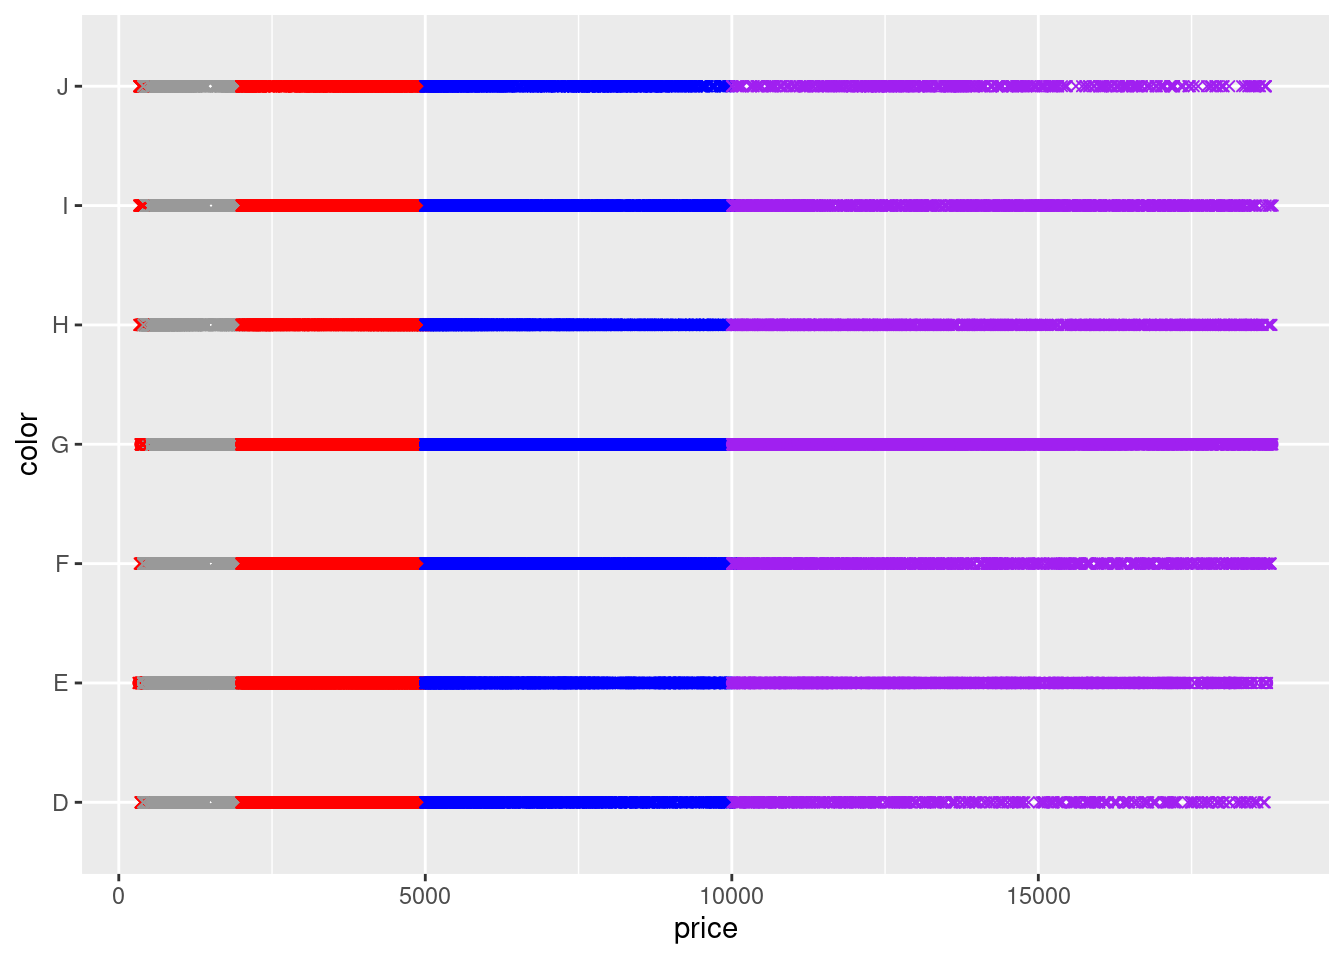
\includegraphics{learningR_files/figure-pdf/unnamed-chunk-4-1.pdf}

\begin{enumerate}
\def\labelenumi{\arabic{enumi})}
\setcounter{enumi}{4}
\tightlist
\item
  source (https://alberts-newsletter.beehiiv.com/){[}{]}
\end{enumerate}

\#tidyselect verbs

contains() starts\_with() ends\_with() 1:10 a:b last\_col() -offset=X
--offset argument matches() num\_range() -needs arguments

based on character names all\_of() any\_of()

pass a formula to check against each column where() -is.numeric()
-is.factor() \textasciitilde mean(.x) \textgreater3.5

\subsection{common tasks---}\label{common-tasks}

apply a function to multiple columns to perform action onto column or
new columns - Across() apply a column of arguments, one by one, as input
into a function - map() apply two or more column of arguments as
simulataneous inputs into a function - map2() apply one column of
arguments as input to function, then combine output with new argument -
purrr::reduce()

apply a function to pairs of columns on a rolling basis (eg. col 1 -2,
col 2 - 3, etc) ????

\section{count}\label{count}

count very useful function to quickly tabulate data use .drop to show
any data that has been filtered out or removed

\begin{Shaded}
\begin{Highlighting}[]
\FunctionTok{library}\NormalTok{(tidyverse)}
\end{Highlighting}
\end{Shaded}

\subsection{how to parse out words from a
sentence}\label{how-to-parse-out-words-from-a-sentence}

\begin{itemize}
\tightlist
\item
  fixed position and fixed seperated but whole word (seperated by
  consistent seperator
\end{itemize}

\begin{Shaded}
\begin{Highlighting}[]
\NormalTok{string }\OtherTok{\textless{}{-}} \FunctionTok{c}\NormalTok{(}\StringTok{"I only want the third word of each sentence"}\NormalTok{,}
            \StringTok{"I only need the third word of each setence"}\NormalTok{,}
            \StringTok{"I only use the third worsd of each sentence"}\NormalTok{)}
\FunctionTok{library}\NormalTok{(tidyverse)}
\NormalTok{stringr}\SpecialCharTok{::}\FunctionTok{word}\NormalTok{(string, }\CommentTok{\#vector of strings}
              \AttributeTok{start=}\DecValTok{3}\NormalTok{, }\CommentTok{\#where to start extraction}
              \AttributeTok{end=}\DecValTok{3}\NormalTok{, }\CommentTok{\#where to end extraction}
              \AttributeTok{sep=}\StringTok{" "}\NormalTok{)}\CommentTok{\# what seperator to parse}
\end{Highlighting}
\end{Shaded}

\begin{verbatim}
[1] "want" "need" "use" 
\end{verbatim}

stringr::word(string,start=x,end=y,sep=?)

is.element(input,check\_strings) -- validates inputs matches at least
one in a set

\chapter{Database and Larger Than Memory
Problems}\label{database-and-larger-than-memory-problems}

\chapter{Resource}\label{resource}

\href{https://smithjd.github.io/sql-pet/chapter-setup-adventureworks-db.html\#}{Resource
to understand databases}

\href{https://r4ds.hadley.nz/databases.html}{R for datascience chapter
on database}

\href{https://dbplyr.tidyverse.org/articles/translation-function.html}{Dbplyr
functions}

\href{https://bwlewis.github.io/duckdb_and_r/talk/talk.html}{How to use
duckdb}

\href{https://dbi.r-dbi.org/}{DBI function overivew}

\href{https://solutions.posit.co/connections/db/}{Posit learning
materials}

\href{https://edgararuiz.github.io/dbplot/}{dbplot\_histogram}

\chapter{Why is this important?}\label{why-is-this-important}

\begin{itemize}
\item
  You will get to a point where the data you need is inside a database
  and not excel sheets or csv files
\item
  This is a point of potential rejoice or mourning
\item
  While we can say goodbye excel sheets and csv files we also need to
  say hello to poorly documented databases, overwhelmed database product
  owners, overworked data engineers, and finally SQL and all of its
  variations
\item
  I recommend you take the time to learn SQL -- the basics are very
  similar to the dplyr commands you already know (slight tweaking of
  evaluation order and syntax) so the beginners learning curve isn't
  steep
\end{itemize}

\begin{tcolorbox}[enhanced jigsaw, title=\textcolor{quarto-callout-note-color}{\faInfo}\hspace{0.5em}{How much SQL should I learn?}, bottomrule=.15mm, titlerule=0mm, left=2mm, rightrule=.15mm, opacityback=0, colframe=quarto-callout-note-color-frame, bottomtitle=1mm, coltitle=black, colback=white, leftrule=.75mm, breakable, colbacktitle=quarto-callout-note-color!10!white, opacitybacktitle=0.6, toprule=.15mm, toptitle=1mm, arc=.35mm]

If you're curious how much SQL you should learn, below is a framework
that I found to be helpful:

\begin{itemize}
\tightlist
\item
  Functions
\end{itemize}

\begin{longtable*}{lll}
\caption*{
{\large Summary of SQL commands and their dplyr counterpart}
} \\ 
\toprule
SQL & dpylr & comment \\ 
\midrule\addlinespace[2.5pt]
where & filter() & can be viewed as one for one replacement to filter(), you can pass arguments with AND or OR,
Sometimes the first argument is TRUE for purely formatting purposes \\ 
select & select() & Can be viewed as one for one replacement for select(), * is short cut for all columns \\ 
group by & group\_by() & can be viewed as one for replacement for group\_by(), you need for it summarization measures as well as partition measures  \\ 
sum & sum() & works the same as sum, na.rm is always TRUE for SQL \\ 
min & min() & works the same as sum, na.rm is always TRUE for SQL \\ 
max & max() & works the same as sum, na.rm is always TRUE for SQL \\ 
count(*) & n() & works similiar to n() \\ 
select distinct & select() |> distinct() & works almost exactly the same \\ 
partition & group\_by() |> mutate() & works exactly the same  \\ 
join & left\_join() & works similiar \\ 
like & str\_detect() & similiar \\ 
top & head() & works the same \\ 
DISTINCT & distinct() & works the same \\ 
DESCRIBE & glimpse() & works simliar, will display the columns and thier data types \\ 
SET &  <-  & works simliar to assign single variables \\ 
BETWEEN & between() & simliar \\ 
MONTH & month() & simliar \\ 
YEAR & year() & simliar \\ 
DAY & day() & simliar \\ 
QUARTER & quarter() & simliar \\ 
DATEDIFF & difftime()  & simliar \\ 
DATETRUC & floor\_date() & similar \\ 
create or replace & tibble() & use this to create the final table \\ 
in &  \%in\% & similiar \\ 
as & rename() & simliar \\ 
with & tibble() & Use this to create CTE or basic mini tables that you can then reference in different steps of the query, makes readable easier \\ 
having & filter() or '[' &  similiar to where \\ 
\bottomrule
\end{longtable*}

There are some nuances, in particular the evaluation order that
typically trip up new SQL users and also some coding conventions that
will be different than what you are used to but in general if you
understand the above R commands you will quickly learn the SQL
counterparts.

With anything, you need to practice! luckily there are multiple SQL
resources and practice studios which can help with reinforcement
learning.

\textbf{Database frameworks}

\begin{itemize}
\item
  Temporary Tables / CTE

  \begin{itemize}
  \tightlist
  \item
    These are tables that only exist when you run them
  \item
    Helpful as interim steps or to break code into subqueries to make it
    more modular
  \end{itemize}
\item
  Curated tables

  \begin{itemize}
  \tightlist
  \item
    Often times you may have loads of raw tables (eg 100s) that you need
    to join together, filter or aggregrate before the data can be usable
  \item
    This process of turning raw /streaming data into table that can be
    consumed for analysis is oftern called data curation
  \item
    This is often times created as a view which can be though of as
    particular snapshot of a table
  \end{itemize}
\item
  Materialized layers

  \begin{itemize}
  \tightlist
  \item
    Materialized layer means the data is more persistent so when you run
    it its not triggering the underlying queries (which will save you
    alot of time)\\
  \item
    Typically you won't know
  \end{itemize}
\end{itemize}

Database structure

\begin{itemize}
\item
  Security Model

  \begin{itemize}
  \tightlist
  \item
    Because data can be privildedged, without a doubt your organization
    has some security model that will aplly row level security and IDs
    to ensure when you access a table you are seeing what you should be
    seeing
  \item
    There is way to much to write here about it and honestly, I'm not
    the right person to answer it
  \end{itemize}
\end{itemize}

You may not need to know any of this but this mostly depends on your
organizations data strategy, staffing levels and operating model

\end{tcolorbox}

\begin{itemize}
\item
  The reason you can survive off of a beginners knowledge base of SQL is
  that luckily there is a life saving package called \texttt{dbplyr}
  that translates your dplyr queries into SQL for you
\item
  It has fairly great coverage but there are limitations which is why
  eventually it will help you to learn some intermediate SQL commands
  and overall database frameworks
\item
  This chapter will go over database essentials and provide resources to
  learn more
\end{itemize}

\section{The Essentials}\label{the-essentials}

\textbf{What do you need to access data in a database?}

\begin{itemize}
\tightlist
\item
  A database with data inside of it\\
\item
  Access / permission to the database
\item
  Location, user name and password to database (or equivalent protocols
  as dictated by your organization's security model)
\item
  Database driver and related utilities
\item
  SQL querys
\item
  Patience
\end{itemize}

\begin{tcolorbox}[enhanced jigsaw, title=\textcolor{quarto-callout-note-color}{\faInfo}\hspace{0.5em}{``What is the advantage of a database?''}, bottomrule=.15mm, titlerule=0mm, left=2mm, rightrule=.15mm, opacityback=0, colframe=quarto-callout-note-color-frame, bottomtitle=1mm, coltitle=black, colback=white, leftrule=.75mm, breakable, colbacktitle=quarto-callout-note-color!10!white, opacitybacktitle=0.6, toprule=.15mm, toptitle=1mm, arc=.35mm]

It comes down to scale and size. At some point your organization or
process will generate substantial data and needs a more structured
process to store the data so that multiple parties can access the data
at scale.

When dealing with a new database some key frameworks are:

\begin{itemize}
\item
  Cloud vs.~On-Premise
\item
  Security model and access
\item
  ``Flavor'' of database
\item
  Improved data management: A database centralizes data, making it
  easier to manage and maintain
\item
  Enhanced data security: A database provides secure storage and
  retrieval of sensitive data through user authentication and access
  control mechanisms
\item
  Better data organization: A database \textbf{theoretically} allows for
  better organization and structure of data through the use of tables,
  indexes, and relationships
\item
  Improved query performance: Databases are optimized for query
  performance, allowing for faster retrieval of data.
\item
  Scalability: Databases can handle large amounts of data and scale as
  needed to meet growing storage demands.
\end{itemize}

Cloud vs On-Premise Database:

\begin{itemize}
\item
  Cloud databases are hosted on remote servers, while on-premise
  databases are hosted on local servers (when you read servers just
  replace it with the word computers. You are either using your
  organization's computer (on prem) or you are using someone else
  (cloud))
\item
  Cloud databases offer greater flexibility in terms of scalability and
  accessibility, as they can be accessed from any location with an
  internet connection.
\item
  On-premise databases provide more control over data security and
  privacy, as the data is stored on a local server and not transmitted
  over the internet.
\item
  Cloud databases typically require less setup and maintenance than
  on-premise databases, as they are managed by the provider.
\item
  Cost: Cloud databases are often subscription-based and can be more
  cost-effective than on-premise databases, especially for small to
  medium-sized businesses.
\end{itemize}

\emph{Security Model and Access:}

\begin{itemize}
\item
  Security model: A database's security model determines who has access
  to the data and how they can access it. Common security models include
  Role-Based Access Control (RBAC), Attribute-Based Access Control
  (ABAC), and Identity-Based Access Control (IBAC).
\item
  Access control: A database's access control mechanisms determine who
  can view, edit, or delete data. This can be based on user
  authentication, role-based access control, or attribute-based access
  control.
\item
  Authentication methods: Databases support various authentication
  methods such as username and password, single sign-on (SSO), and
  two-factor authentication (2FA).
\item
  Authorization methods: Databases support various authorization methods
  such as row-level security, column-level security, and table-level
  security.
\item
  Auditing and logging: Databases can log all access attempts and
  successful accesses to track user activity and detect potential
  security breaches.
\item
  Encryption: Databases can encrypt data both in transit and at rest to
  protect it from unauthorized access.
\item
  Backup and recovery: Databases provide mechanisms for backing up data
  and recovering from failures or security incidents.
\item
  Identity and access management (IAM): IAM systems manage user
  identities and access rights within the database, ensuring that only
  authorized users can access the data.
\item
  Role-based access control (RBAC): RBAC allows for assigning roles to
  users based on their job function or responsibilities, limiting the
  data they have access to.
\item
  Attribute-based access control (ABAC): ABAC grants or denies access to
  data based on attributes associated with the user or the data itself,
  such as location or time of day.
\end{itemize}

\end{tcolorbox}

\textbf{What does a database need from you?}

\begin{itemize}
\item
  The most frustrating part of database is getting access to the
  database, setting up the database utilities and then making the
  initial connection
\item
  There are multiple ways to connect to a database however almost all
  require the following:

  \begin{itemize}
  \tightlist
  \item
    User name
  \item
    Password
  \item
    Database driver
  \item
    Connection string and associated arguments
  \item
    SQL query
  \end{itemize}
\item
  We will review the DSN method for connecting to a database
\item
  These tend to be confusing because much of this is controlled and
  managed by your local IT department so whatever documentation or guide
  you read on online may not translate one for one to your localized
  experienced (this includes this guide as well :(
\end{itemize}

\section{Set up ODBC Driver}\label{set-up-odbc-driver}

\begin{itemize}
\item
  Download (if required) a database driver for your database -- this is
  typically on the database company's website

  \begin{itemize}
  \tightlist
  \item
    Your company may have centralized package manager system where you
    will need to download and install all required drivers via that
    packet manager
  \end{itemize}
\item
  Configure your DSN so that you can be authenticated
\item
  Your database platform should have documentation on how to do this and
  your internal IT team \textbf{should} be able to articulate any proxy
  / security requirements
\item
  Here is some example
  \href{https://docs.snowflake.com/en/developer-guide/odbc/odbc-windows}{documentation}
\item
  You are essentially saving the required information (listed above) to
  your computer so that you can pass these arguments to the database
\item
  Pay attention to the name you setup the DSN driver, you will need this
  later one
\end{itemize}

\textbf{Example Paramaters are below}

\begin{itemize}
\tightlist
\item
  User
\item
  Password
\item
  Server
\item
  Database
\item
  Schema
\item
  Warehouse\\
\item
  Tracing
\item
  Authenticator
\end{itemize}

\section{Create Connection String}\label{create-connection-string}

\begin{itemize}
\item
  If the above is done correctly you can then use DBI package in R to
  connect to the database of your choice
\item
  Create a connection string with DBI::dbConnect()

  \begin{itemize}
  \item
    Select the DBMS wtih the driver\_name such as ODBC::ODBC() to access
    your DSN set up connect to external database or can use DMBS package
    such as duckdb::duckdb() to replicate an internal instance of a
    database
  \item
    DSN name if external database (the name used to set up ODBC driver)
  \item
    Alternatively, you can directly supply the arguments in
    DBI::dbConnect() such as hostname,port,username, etc
  \end{itemize}
\end{itemize}

\begin{Shaded}
\begin{Highlighting}[]
\DocumentationTok{\#\# this uses duckdb example to create a connection string}

\NormalTok{con }\OtherTok{\textless{}{-}}\NormalTok{ DBI}\SpecialCharTok{::}\FunctionTok{dbConnect}\NormalTok{(}\AttributeTok{drv=}\NormalTok{duckdb}\SpecialCharTok{::}\FunctionTok{duckdb}\NormalTok{())}

\DocumentationTok{\#\# this is alternative example using a made up DSN name }

\NormalTok{con  }\OtherTok{\textless{}{-}}\NormalTok{ DBI}\SpecialCharTok{::}\FunctionTok{dbConnect}\NormalTok{(}
  \AttributeTok{drv=}\NormalTok{odbc}\SpecialCharTok{:}\FunctionTok{odbc}\NormalTok{()}
\NormalTok{  ,}\AttributeTok{dsn=}\StringTok{"your\_DSN\_name"} 
\NormalTok{  )}
\end{Highlighting}
\end{Shaded}

\begin{tcolorbox}[enhanced jigsaw, title=\textcolor{quarto-callout-note-color}{\faInfo}\hspace{0.5em}{Additional Utilities}, bottomrule=.15mm, titlerule=0mm, left=2mm, rightrule=.15mm, opacityback=0, colframe=quarto-callout-note-color-frame, bottomtitle=1mm, coltitle=black, colback=white, leftrule=.75mm, breakable, colbacktitle=quarto-callout-note-color!10!white, opacitybacktitle=0.6, toprule=.15mm, toptitle=1mm, arc=.35mm]

\begin{itemize}
\tightlist
\item
  the DBI and ODBC packages are extremely useful for database related
  utilities
\item
  While they have some existing overlap, they can be used to view the
  schema in your database, list active connections and also disconnect.
\item
  Below are some useful utilities:
\end{itemize}

\subsubsection{list your drivers}\label{list-your-drivers}

odbc::odbcListDrivers()

\subsubsection{list active connections}\label{list-active-connections}

DBI::dbListConnections()

\section{Checks if you can connect}\label{checks-if-you-can-connect}

DBI::dbCanConnect()

\section{List tables listed under
connection}\label{list-tables-listed-under-connection}

DBI::dbListTables()

\subsection{list tables in connection}\label{list-tables-in-connection}

\texttt{dbListTables(con)} to list tables associated with a connection

\end{tcolorbox}

\begin{itemize}
\tightlist
\item
  After you have created a connection string you now need to retrieve
  information from the database
\end{itemize}

\section{Option 1: Create SQL string}\label{option-1-create-sql-string}

\begin{itemize}
\item
  If you know the database, schema and table name that you want, you can
  write the initial sql query to connect to the database
\item
  You can write simple or advance query insde the \texttt{dplyr::sql()}
  function
\end{itemize}

\begin{Shaded}
\begin{Highlighting}[]
\NormalTok{sql\_query }\OtherTok{\textless{}{-}}\NormalTok{ dplyr}\SpecialCharTok{::}\FunctionTok{SQL}\NormalTok{(}\StringTok{"select *  from database\_name"}\NormalTok{)}
\end{Highlighting}
\end{Shaded}

\section{Accessing Databse}\label{accessing-databse}

\begin{itemize}
\tightlist
\item
  Use connection string and sql query together to create a lazy table
  with \texttt{dplyr::tbl()}
\item
  We call this a lazy table because it won't actually execute the query
  and return the results which is good because your query might return
  100s of results
\end{itemize}

\begin{Shaded}
\begin{Highlighting}[]
\NormalTok{data\_db }\OtherTok{\textless{}{-}}\NormalTok{ dplyr}\SpecialCharTok{::}\FunctionTok{tbl}\NormalTok{(con,sql\_query)}
\end{Highlighting}
\end{Shaded}

\begin{itemize}
\item
  From there you can use \emph{dplyr} back end queries to see everything
  (notice the distinction betwee \textbf{db}pyr and dplyr
\item
  If you use the dbplyr package, you are limited to queries that can be
  translated to sql which are detailed below

  \begin{itemize}
  \tightlist
  \item
    \href{https://github.com/tidyverse/dbplyr/blob/main/R/backend-.R}{github
    of dplyr commands that can be used in dbplyr}
  \item
    You can also check the database
    specific\href{\%5Bhttps://github.com/tidyverse/dbplyr/blob/main/R/backend-snowflake.R}{here}
  \end{itemize}
\item
  You can see what query it will generate with
  \texttt{dbplyr::show\_query()}
\item
  Notice the class of the object you return, you are returning a
  database object -- if you want to return a dataframe you need to use
  \texttt{dplyr::collect()}
\end{itemize}

\section{Option 2: Push existing data into a
database}\label{option-2-push-existing-data-into-a-database}

\begin{itemize}
\item
  First you need to have a connection string to a database (and write
  permissions)
\item
  If you already have something as a dataframe you can upload it to a
  database with DBI::dbWriteTable(con,``tbl\_name'',df) which will write
  the table to the connection with the name you gave

  \begin{itemize}
  \tightlist
  \item
    DBI::dbWriteTable() can write a r dataframe or you can use sql to
    create a virtual table if you want
  \item
    dbplyr::copy\_inline(con\_db,df = df) is alternative method
  \item
    If you have duckdb connection you can use the
    duckdb::duckdb\_register()
  \end{itemize}
\end{itemize}

\begin{Shaded}
\begin{Highlighting}[]
\CommentTok{\# create connection}
\NormalTok{con\_db }\OtherTok{\textless{}{-}}\NormalTok{ DBI}\SpecialCharTok{::}\FunctionTok{dbConnect}\NormalTok{(duckdb}\SpecialCharTok{::}\FunctionTok{duckdb}\NormalTok{())}

\CommentTok{\# write data into database}
\NormalTok{DBI}\SpecialCharTok{::}\FunctionTok{dbWriteTable}\NormalTok{(con\_db,}\AttributeTok{name =} \StringTok{"diamonds\_db"}\NormalTok{,}\AttributeTok{value =}\NormalTok{ ggplot2}\SpecialCharTok{::}\NormalTok{diamonds)}

\CommentTok{\# or alternative use the database argument to regester}
\NormalTok{duckdb}\SpecialCharTok{::}\FunctionTok{duckdb\_register}\NormalTok{(con\_db, }\StringTok{"diamonds\_db\_2"}\NormalTok{,}\AttributeTok{df =}\NormalTok{  ggplot2}\SpecialCharTok{::}\NormalTok{diamonds)}

\CommentTok{\# validate data is in database by reference connection}
\NormalTok{DBI}\SpecialCharTok{::}\FunctionTok{dbListTables}\NormalTok{(con\_db)}
\end{Highlighting}
\end{Shaded}

\begin{verbatim}
[1] "diamonds_db"   "diamonds_db_2"
\end{verbatim}

\begin{Shaded}
\begin{Highlighting}[]
\CommentTok{\# Pull in data in database format}
\NormalTok{diamonds\_db }\OtherTok{\textless{}{-}}\NormalTok{ dplyr}\SpecialCharTok{::}\FunctionTok{tbl}\NormalTok{(con\_db,}\StringTok{"diamonds\_db"}\NormalTok{)}
\end{Highlighting}
\end{Shaded}

\section{What happens if dbplyr doesn't have a function that I
need?}\label{what-happens-if-dbplyr-doesnt-have-a-function-that-i-need}

\subsection{built in helper functions}\label{built-in-helper-functions}

\subsection{create sql query and use
it}\label{create-sql-query-and-use-it}

\section{how can I build a package for
this?}\label{how-can-i-build-a-package-for-this}

\subsection{sprintf() and SQL}\label{sprintf-and-sql}

\subsection{dbplyr}\label{dbplyr}

\section{Putting it all together}\label{putting-it-all-together}

\begin{itemize}
\tightlist
\item
  Set up your drive, get required database info and related utilities
\item
  Create connection to your database
\item
  write an inital query to select the columns that you want or need
\item
  Use dbplyr to translate dplyr queries to SQL
\item
  return results to your local machine with dplyr::collect()
\end{itemize}

\chapter{Larger than memory problems}\label{larger-than-memory-problems}

\begin{itemize}
\item
  Sometimes you don't have a database but have data that is larger than
  memory
\item
  Luckily, you don't need a database to take advantage of the tricks we
  have learnt to move solve your data larger than memomory problems
\item
  Sometimes you may not have a database to connect to and instead have a
  very large csv file or dataframes
\item
  There are two packages that are exceptionally helpful here

  \begin{itemize}
  \tightlist
  \item
    duckdb() and arrow()
  \end{itemize}
\item
  This isn't the technically correct response but duckdb() allows you to
  build an in memory database whereas arrow compresses your information
  into some sort of parquet type structure
\item
  What makes these so great is that dbplyr will translate your dplyr
  commands to either duckdb or arrow language
\item
  Some dplyr functions are avaialble in one package that aren't
  avaialble in the other
\item
  However you can pass an object from duckdb to arrow as much as you
  want
\end{itemize}

\textbf{What is key difference?}

\begin{itemize}
\tightlist
\item
  Duckdb will return first 1000 rows of your query so you can check if
  your query worked well, whereas arrow won't let you see it (including
  if your query returns an error which can be annoying)
\end{itemize}

To understand how to use the packages,let us define two scenarios:

\begin{enumerate}
\def\labelenumi{\arabic{enumi})}
\tightlist
\item
  You have a lot of csv files that you need to upload and analyze
\item
  As a result of simulation of some other you have multiple tables that
  seperately are okay but together are generating you have very large
  dataframe that you need to join together to analyze and manipulate
\item
  You have interim data that you want to save in workflow that is large
\end{enumerate}

\subsection{Large csv files that you need to work
with:}\label{large-csv-files-that-you-need-to-work-with}

\begin{itemize}
\tightlist
\item
  If you have large offline files you can quickly easily load this into
  duckdb with \texttt{duckdb\_read\_csv()} or the collection of arrow
  functions (eg. \texttt{arrow::read\_csv\_arrow()}).
\end{itemize}

Arrow will support json, feather, delimiter, parquet, or csv amongst
other whereas duckdb only supports csv (if not already an object)

\begin{itemize}
\tightlist
\item
  This will load the csv files directly to your duck db in memory
  database
\item
  You first need to create connection string
\end{itemize}

\subsection{Existing dataframes (however they got there) that are either
too
large}\label{existing-dataframes-however-they-got-there-that-are-either-too-large}

or individually are okay but seperately aren't okay

\begin{itemize}
\tightlist
\item
  You first need to get your data into R as a dataframe
\item
  Then you need to register your dataframe to your in duckdb memory
  database
\item
  From there you can move the datafrme from duckdb to arrow as you would
  like
\end{itemize}

\chapter{Special tricks}\label{special-tricks}

\section{You can pass one database object to
duckdb}\label{you-can-pass-one-database-object-to-duckdb}

\begin{Shaded}
\begin{Highlighting}[]
\InformationTok{\textasciigrave{}\textasciigrave{}\textasciigrave{}\{r\}}
\InformationTok{\#| label: db{-}connect example}
\InformationTok{\#| eval: true}

\InformationTok{\#\# create connection string locally}
\InformationTok{con\_db \textless{}{-} DBI::dbConnect(duckdb::duckdb())}

\InformationTok{\# loads data into your connection either in memory}
\InformationTok{DBI::dbWriteTable(con\_db,"diamonds\_db",ggplot2::diamonds)}

\InformationTok{\#create new table to the connection}

\InformationTok{DBI::dbExecute(con\_db, "CREATE TABLE duckdb\_table (col1 INT, col2 STRING)")}
\InformationTok{\textasciigrave{}\textasciigrave{}\textasciigrave{}}
\end{Highlighting}
\end{Shaded}

\begin{verbatim}
[1] 0
\end{verbatim}

\#preview what is in your connection

\begin{Shaded}
\begin{Highlighting}[]
\NormalTok{DBI}\SpecialCharTok{::}\FunctionTok{dbListTables}\NormalTok{(con\_db)}

\NormalTok{dbplyr}\SpecialCharTok{::}\FunctionTok{copy\_inline}\NormalTok{(con\_db,}\AttributeTok{df =}\NormalTok{ diamonds)}


\NormalTok{diamonds\_db }\OtherTok{\textless{}{-}}\NormalTok{ dplyr}\SpecialCharTok{::}\FunctionTok{tbl}\NormalTok{(con\_db}
\NormalTok{    ,}\StringTok{"diamonds\_db"}
\NormalTok{    )}
\end{Highlighting}
\end{Shaded}

\chapter{Example of passing one database object to
arrow}\label{example-of-passing-one-database-object-to-arrow}

\begin{Shaded}
\begin{Highlighting}[]
\NormalTok{diamonds\_db }\SpecialCharTok{\%\textgreater{}\%} 
  
  \FunctionTok{mutate}\NormalTok{(}\AttributeTok{good\_indicator=}\FunctionTok{if\_else}\NormalTok{(cut}\SpecialCharTok{==}\StringTok{"Good"}\NormalTok{,}\DecValTok{1}\NormalTok{,}\DecValTok{0}\NormalTok{)) }\SpecialCharTok{\%\textgreater{}\%}
  \FunctionTok{group\_by}\NormalTok{(color) }\SpecialCharTok{\%\textgreater{}\%} 
  \FunctionTok{summarise}\NormalTok{(}
    \AttributeTok{n=}\FunctionTok{n}\NormalTok{()}
\NormalTok{    ,}\AttributeTok{mean=}\FunctionTok{mean}\NormalTok{(carat)}
\NormalTok{    ,}\AttributeTok{mean\_price=}\FunctionTok{mean}\NormalTok{(price)}
\NormalTok{    ,}\AttributeTok{mean\_ind=}\FunctionTok{mean}\NormalTok{(good\_indicator)}
\NormalTok{    ,}\AttributeTok{mean\_adj=}\FunctionTok{mean}\NormalTok{(carat[good\_indicator}\SpecialCharTok{==}\DecValTok{1}\NormalTok{])}
\NormalTok{  ) }\SpecialCharTok{\%\textgreater{}\%} 

  \FunctionTok{arrange}\NormalTok{(}\FunctionTok{desc}\NormalTok{(color)) }\SpecialCharTok{\%\textgreater{}\%} 
  \FunctionTok{mutate}\NormalTok{(}\AttributeTok{rolling\_price=}\FunctionTok{cumsum}\NormalTok{(mean\_price)) }\SpecialCharTok{\%\textgreater{}\%} 
\NormalTok{    arrow}\SpecialCharTok{::}\FunctionTok{to\_arrow}\NormalTok{() }\SpecialCharTok{\%\textgreater{}\%} 
  \FunctionTok{ungroup}\NormalTok{() }\SpecialCharTok{\%\textgreater{}\%} 
 \FunctionTok{filter}\NormalTok{(color}\SpecialCharTok{==}\StringTok{"H"}\NormalTok{) }\SpecialCharTok{\%\textgreater{}\%} 
  \FunctionTok{select}\NormalTok{(color,mean\_adj) }\SpecialCharTok{\%\textgreater{}\%} 
  \FunctionTok{collect}\NormalTok{()}
\end{Highlighting}
\end{Shaded}

\chapter{Additional tricks}\label{additional-tricks}

\subsection{Running SQL in R}\label{running-sql-in-r}

\begin{itemize}
\tightlist
\item
  If you are using rmakrdown or quarto, you can run the sql query in a
  window and have it results saved as a datafarme
\end{itemize}

\begin{Shaded}
\begin{Highlighting}[]
\KeywordTok{SELECT} \OperatorTok{*} 

\KeywordTok{FROM}\NormalTok{ diamonds\_db}

\KeywordTok{WHERE}\NormalTok{ cut}\OperatorTok{==}\StringTok{\textquotesingle{}Good\textquotesingle{}}

\KeywordTok{LIMIT} \DecValTok{100}
\end{Highlighting}
\end{Shaded}

\begin{itemize}
\tightlist
\item
  If you want to run it in rmarkdown, you can do the following
\end{itemize}

\begin{Shaded}
\begin{Highlighting}[]

\KeywordTok{SELECT} \OperatorTok{*} 

\KeywordTok{FROM}\NormalTok{ diamonds\_db}

\KeywordTok{WHERE}\NormalTok{ cut}\OperatorTok{==}\StringTok{\textquotesingle{}Good\textquotesingle{}}

\KeywordTok{LIMIT} \DecValTok{100}
\end{Highlighting}
\end{Shaded}

\section{Run SQL queries safely}\label{run-sql-queries-safely}

\section{How to plot a database
object}\label{how-to-plot-a-database-object}

\section{How to build packages or function to access
dbplyr}\label{how-to-build-packages-or-function-to-access-dbplyr}

\begin{itemize}
\item
  two options:

  \begin{itemize}
  \tightlist
  \item
    sprintf to generate actual sql queries
  \item
    dbplyr / similiar to spring
  \end{itemize}
\end{itemize}



\end{document}
